% $Header: /home/nthiery/CVSROOT/www/qualification/talk.tex,v 1.1 2011-06-27 08:15:50 nthiery Exp $

% Ajouter l'exemple de la factorisation

% Distinction Parent / Element / Morphisme

% En live dans le notebook: Groupes / Semigroupes

% Categories pour éviter la duplication

% Problème 2: passage à l'échelle (axiomes / constructions fonctorielles)

% Problème: C3 (récupérer des bouts de Pycon)

% Autre approche: GAP

% Ouvertures:

% - Comment tirer parti des multiméthodes?

% - Compilation?

% - Problèmes similaires dans les systèmes de preuves

% - Systèmes de modélisation des connaissances mathématiques

%   Modéliser plus explicitement => interfaces entres systèmes

% - Bourse de thèse

\documentclass[%compress,
%handout
]{beamer}

\mode<presentation>
{
 \usetheme{Singapore}
 \setbeamercovered{transparent}
\setbeamersize{text margin left =1.2cm}
\setbeamersize{text margin right=0.8cm}
\setbeamertemplate{navigation symbols}{}
}



\usepackage[utf8]{inputenc}
\usepackage[francais,english]{babel}
\usepackage[babel=true,kerning=true]{microtype}
%\usepackage[left=1cm]{geometry}
\usepackage{listings}
%\usepackage{times}
\usepackage[T1]{fontenc}
%\usepackage{amssymb}
\usepackage{amsmath}
\usepackage{amsthm}
\usepackage{hyperref}
\usepackage{ae,aecompl}         % Use (almost) Type 1 fonts
\usepackage{ifthen}
\usepackage{ulem}
\usepackage{listings}
\lstset{
  numbers=none,
  frame=leftline,
  framerule=.5ex,
  framesep=1ex,
  rulecolor=\color{gray!30},
  xleftmargin=2ex,
  %aboveskip=2pt,
  %basicstyle={\color{black}}
  basicstyle={\ttfamily\small},
  columns=fixed,
  showstringspaces=false,
  commentstyle={\ttfamily\color{DarkRed}},
  keywordstyle={\ttfamily\color{DarkBlue}},
  stringstyle={\ttfamily\color{DarkGreen}},
  fontadjust=true,
  %basewidth={1.22ex},
  basewidth={1.09ex},
  breaklines=false,
  basewidth={1.09ex},
  %backgroundcolor=LightBlue,
  literate={é}{{\'e}}1 {è}{{\`e}}1 {à}{{\`a}}1 {î}{{\^i}}1 {ê}{{\^e}}1 {ô}{{\^o}}1 {û}{{\^u}}1
           {sage:}{{{\scalebox{.9}[1]{\ttfamily\bfseries\color{DarkBlue}{sage:}}}}}5
           {...\ \ }{{{\ttfamily\bfseries\color{DarkBlue}{...\ \ }}}}5,
}

\usepackage{xspace}
\usepackage{calc}
%\usepackage[usenames,svgnames]{xcolor}
\usepackage{tikz}
\definecolor{DarkRed}{RGB}{200,0,0}
\definecolor{DarkGreen}{RGB}{0,100,0}
\definecolor{DarkBlue}{RGB}{0,0,255}
\definecolor{green}{RGB}{0,150,0}

\usepackage{graphicx}
\graphicspath{{Pictures/}}

\newcommand{\fr}[1]{}
\newcommand{\en}[1]{#1}

\title{\fr{Infrastructure pour du code générique dans \SageMath:
    catégories, axiomes, constructions, ...}
  \en{Modeling mathematics in Python \& SageMath: some fun challenges}
}

\author{\Large Nicolas M. Thiéry}

\institute{LRI, Université Paris Sud 11}

\date{October 8th of 2018, PyData, Paris}

% Used in the figures to latex them separately
\newenvironment{previewthispiece}{}{}

\usepackage{verbatim}

%%%%%%%%%%%%%%%%%%%%%%%%%%%%%%%%%%%%%%%%%%%%%%%%%%%%%%%%%%%%%%%%%%%%%%%%%%%%%%
% Tiré de /usr/lib/texmf/texmf/doc/help/faq/FAQ_LaTeX_francaise_V1.8
%%% ----------debut de bigcenter.sty--------------

%%% nouvel environnement bigcenter
%%% pour centrer sur toute la page (sans overfull)

\makeatletter
\newskip\@bigflushglue \@bigflushglue = -100pt plus 1fil

\def\bigcenter{\trivlist \bigcentering\item\relax}
\def\bigcentering{\let\\\@centercr\rightskip\@bigflushglue%
\leftskip\@bigflushglue
\parindent\z@\parfillskip\z@skip}
\def\endbigcenter{\endtrivlist}
\makeatother

%%%%%%%%%%%%%%%%%%%%%%%%%%%%%%%%%%%%%%%%%%%%%%%%%%%%%%%%%%%%%%%%%%%%%%%%%%%%%%

\newcommand{\TODO}[1]{}
%\newcommand{\TODO}[1]{\marginpar{\small To do: #1}}
\newcommand{\FIXME}[1]{}
%\newcommand{\FIXME}[1]{\marginpar{\small Fix me: #1}}

%%%%%%%%%%%%%%%%%%%%%%%%%%%%%%%%%%%%%%%%%%%%%%%%%%%%%%%%%%%%%%%%%%%%%%%%%%%%%%
% Macros diverses

\renewcommand{\k}{{\mathbb{C}}} % MAYBE CHANGE BACK TO \K?
\newcommand{\realring}{{\mathbb{K}}}
\newcommand{\NN}{{\mathbb{N}}}
\newcommand{\F}{{\mathbb{F}}}
\newcommand{\CC}{{\mathbb{C}}}
\newcommand{\ZZ}{{\mathbb{Z}}}
\newcommand{\QQ}{{\mathbb{Q}}}
\newcommand{\RR}{{\mathbb{R}}}
\newcommand{\KK}{{\mathbb{K}}}
\newcommand{\s}{w}
\renewcommand{\t}{{w'}}
\newcommand{\End}{{\operatorname{End}}}
\newcommand{\sym}{{\operatorname{Sym}}}
\newcommand{\qsym}{{\operatorname{QSym}}}
\newcommand{\ncsf}{{\operatorname{NCSF}}}

\renewcommand{\RR}{\mathcal{R}}
\newcommand{\LL}{\mathcal{L}}
\newcommand{\JJ}{\mathcal{J}}
\newcommand{\HH}{\mathcal{H}}
\newcommand{\BB}{\mathcal{B}}

\newcommand{\geh}{\mathfrak{g}}
\newcommand{\wt}{\mathrm{wt}}
\newcommand{\D}{\Pi}

\newcommand{\ip}[1]{\langle #1 \rangle}
\newcommand{\af}{\mathrm{af}}
\newcommand{\init}{{\operatorname{init}}}
\newcommand{\id}{{\operatorname{id}}}
\newcommand{\im}{{\operatorname{im}}}
\newcommand{\rank}{{\operatorname{rank}}}
\newcommand{\sign}{{\operatorname{sign}}}
\newcommand{\powerset}{{\mathcal{P}}}
\newcommand{\multinomial}{{\operatorname{multinomial}}}
\newcommand{\size}{{\operatorname{size}}}
\newcommand{\rad}{{\operatorname{rad}}}
%\newcommand{\hom}{{\operatorname{Hom}}}
%\newcommand{\ker}{{\operatorname{ker}}}

\newcommand{\suchthat}{{\ |\ }}

\newcommand{\starcombinat}{\href{http://wiki.sagemath.org/combinat/}{{\raisebox{-.1ex}{$\ast$}\text{-Combinat}}}\xspace}
\newcommand{\starcombinatsimple}{\href{http://wiki.sagemath.org/combinat/}{$\ast$\text{-Combinat}}\xspace}
\newcommand{\sagecombinat}{\href{http://wiki.sagemath.org/combinat/}{\texttt{Sage-Combinat}}\xspace}
\newcommand{\Sage}{\texttt{Sage}\xspace}
\newcommand{\SageMath}{\texttt{SageMath}\xspace}
\newcommand{\mupad}{\texttt{MuPAD}\xspace}
\newcommand{\mupadcombinat}{\href{http://mupad-combinat.sf.net/}{\texttt{MuPAD-Combinat}}\xspace}

\newcommand{\blue}[1]{{\color{blue}#1}}

\begin{document}

\begin{frame}
  \vspace{-.5cm}
  \titlepage
  \begin{bigcenter}
    \vspace{-.5cm}
    \includegraphics[height=5cm,angle=90]{Pictures/G2-alcove-path.pdf}\qquad
    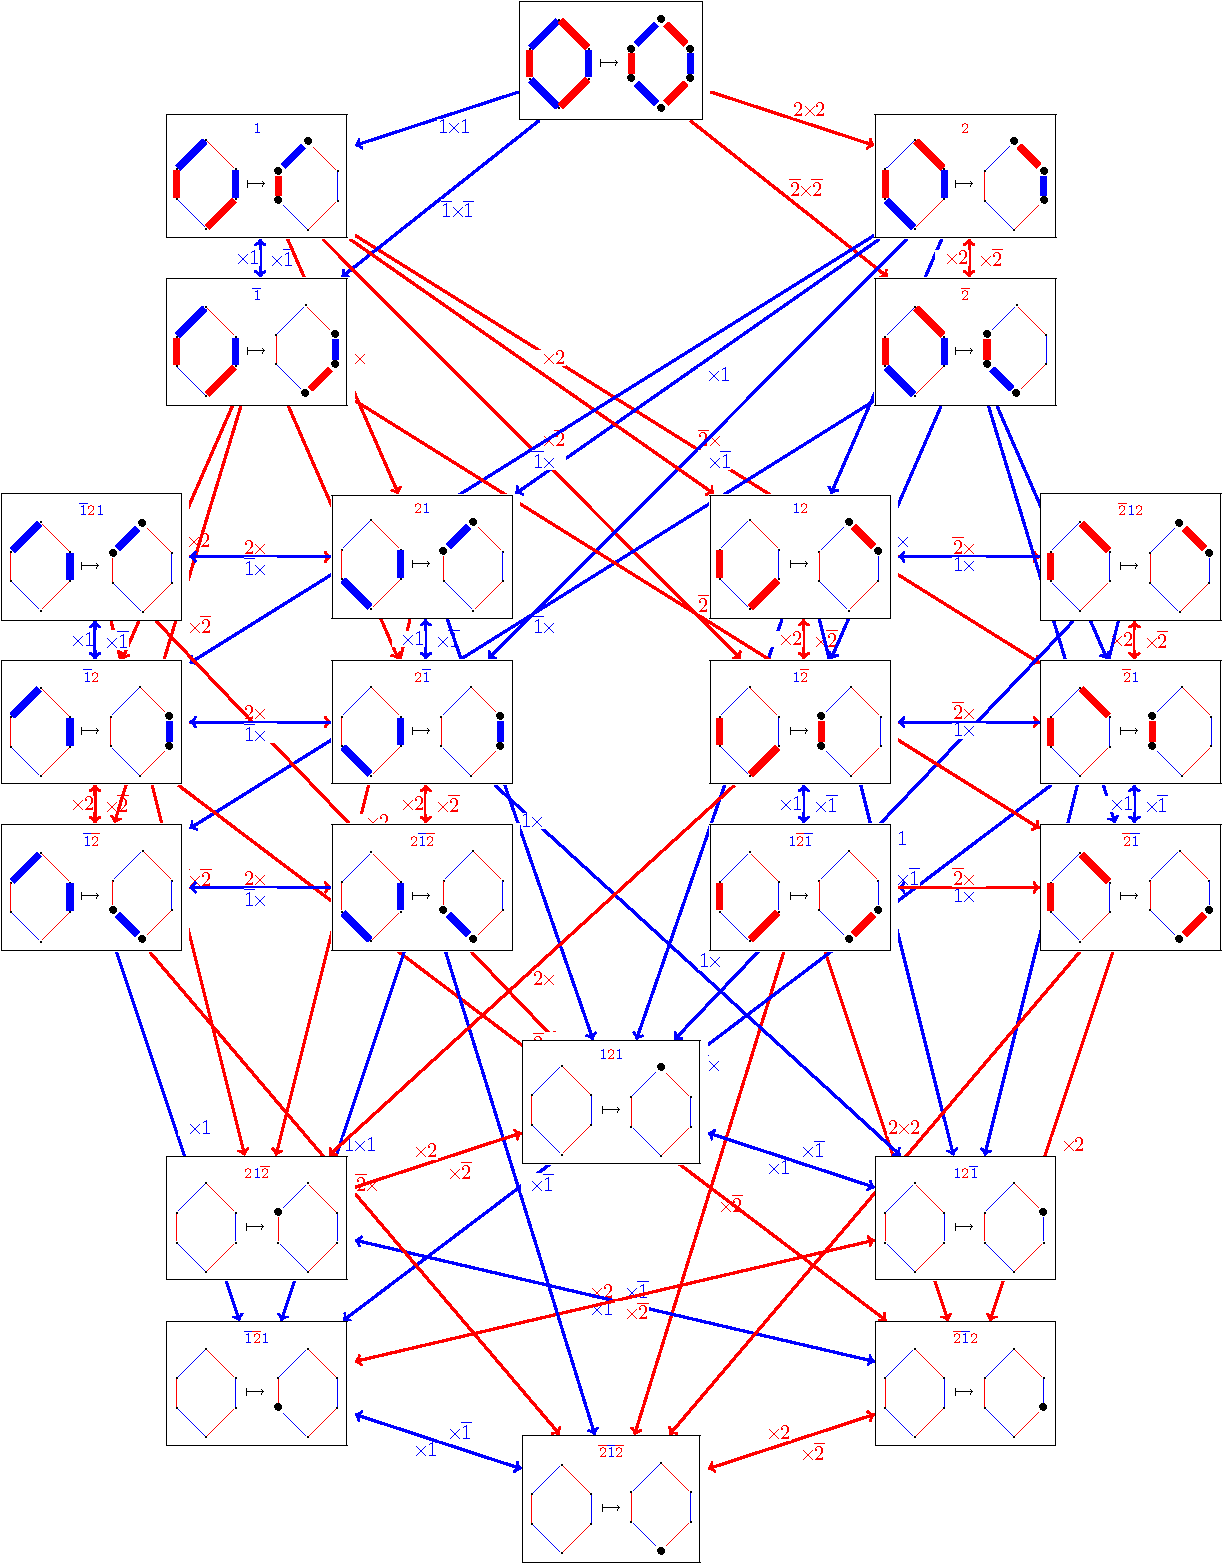
\includegraphics[height=5cm,angle=90]{Pictures/J-graph-A2.pdf}
  \end{bigcenter}
\end{frame}

\begin{frame}{\fr{Résumé}\en{Abstract}}
  \fr{Le logiciel libre \SageMath permet de manipuler des milliers
    d'objets mathématiques différents avec des dizaines de milliers de
    fonctions.  Un système de cette taille requiert une infrastructure
    permettant l'écriture et l'organisation de code, de documentation
    et de tests génériques s'appliquant uniformément à tous les objets
    satisfaisant certaines propriétés.}
  %
  \en{The \SageMath systems provides thousands of mathematical objects
    and tens of thousands of operations to compute with them. A system
    of this scale requires an infrastructure for writing and
    structuring generic code, documentation, and tests that apply
    uniformly on all objects within certain realms.}

  \fr{Dans cet exposé, nous décrirons l'infrastructure implantée dans
    \SageMath -- qui s'appuie sur la programmation objet classique en
    Python, avec des mécanismes pour passer à l'échelle (classes
    dynamiques, mixins, ...) s'appuyant sur la forte sémantique
    disponible (catégories, axiomes, constructions) -- et la
    comparerons avec ce qui est fait dans d'autres systèmes.}

  \en{In this talk, we describe the infrastructure implemented in
    \SageMath. It is based on the standard object oriented features of
    Python, together with mechanisms to scale (dynamic classes,
    mixins, ...) thanks to the rich available semantic (categories,
    axioms, constructions). We relate the approach taken with that in
    other systems, and discuss work in progress}
\end{frame}

% \section{\SageMath}

% \begin{frame}{\SageMath{}: \url{sagemath.org}}

%   \begin{block}{Mission}
%     « \emph{Créer une alternative libre et viable à
%       Maple\texttrademark{}, Mathematica\texttrademark{},
%       Magma\texttrademark{} et MATLAB\texttrademark{} }»
%   \end{block}
%   \pause
%   \bigskip

%   \begin{block}{\fr{En quelques chiffres}\en{In a nutshell}}
%     \begin{itemize}
%     \item Initié en 2004 par William Stein
%     \item Basé sur NumPy, SciPy, matplotlib, Sympy, Maxima, GAP,
%       FLINT, Singular, R, ...
%     \item 40000 utilisateurs?
%     \item 200 contributeurs
%     \end{itemize}
%   \end{block}
% \end{frame}

\section{SageMath}

\begin{frame}{Computational Pure Mathematics!}
  \only<1>{\centerline{\Large Maple? Mathematica?}}
  \visible<2->{
  \only<2->{\centerline{\Large \sout{Maple}, \sout{Mathematica}}}
  \bigskip
  \medskip
  \centerline{\Huge\url{sagemath.org}}
  \bigskip
  \pause
  \pause
  \begin{itemize}
  \item Open source
  \item Based on \textbf{Python} + hundreds of specialized libraries:\\
    Algebra, Combinatorics, Number Theory, Cryptography, ...
  \item Plays well with the Scientific Python stack
    \pause
  \item 200+ regular contributors
  \item Workshops: \textbf{Sage Days 97!}
    \pause
  \item SageMath notebook inspired the Jupyter notebook
  \item Cython originally developed for SageMath
  \end{itemize}}
\end{frame}

\begin{frame}[fragile]{\SageMath: \fr{un logiciel de calcul
      mathématique}\en{a general purpose software for mathematics}}
  \pause
  \blue{\fr{Nombres}\en{Numbers}:}\quad $42$, $\frac79$, $\frac{I+sqrt(3)}2$, $\pi$, $2.71828182845904523536028747?$
  \bigskip\pause

  \blue{Matrices:}
  $\left(\begin{array}{rrrr}
      4 & -1 & 1 & -1 \\
      -1 & 2 & -1 & -1 \\
      0 & 5 & 1 & 3
    \end{array}\right)$,
  $\left(\begin{array}{rrr}
      1.000 & 0.500 & 0.333 \\
      0.500 & 0.333 & 0.250 \\
      0.333 & 0.250 & 0.200
    \end{array}\right)$

  \bigskip\pause

  \blue{\fr{Polynômes}\en{Polynomials}:}\quad $-9x^{8} + x^{7} + x^{6} - 13x^{5} - x^{3} - 3x^{2} - 8x + 4$ %\sage{ZZ[x].random_element(degree=8)}$
  \bigskip\pause

  \blue{\fr{Séries}\en{Series}:}\quad $1 + 1 x + \frac{1}{2} x^{2} + \frac{1}{6} x^{3} + \frac{1}{24} x^{4} + \frac{1}{120} x^{5} + \cdots$
  % \sage{exp(x).series(x,6)}$
  \bigskip\pause

  \blue{\fr{Expressions symboliques, équations}\en{Symbolic expressions, equations}:}\quad $cos(x)^2 + sin(x)^2 == 1$

  \bigskip\pause

  \blue{\fr{Corps finis, extensions algébriques, courbes elliptiques, ...}
  \en{Finite fields, algebraic extensions, elliptic curves, ...}}

\end{frame}

\def\lr#1{\multicolumn{1}{|@{\hspace{.6ex}}c@{\hspace{.6ex}}|}{\raisebox{-.3ex}{$#1$}}}
\begin{frame}[fragile]{\fr{Objets combinatoires}\en{Combinatorial objects}}
  \begin{bigcenter}

    \raisebox{2ex}{$\begin{array}[b]{*{4}c}\cline{1-4}
        \lr{1}&\lr{3}&\lr{4}&\lr{7}\\\cline{1-4}
        \lr{2}&\lr{5}&\lr{6}\\\cline{1-3}
        \lr{8}\\\cline{1-1}
      \end{array}$}
    \qquad
    \scalebox{.7}{{\setlength\unitlength{4mm}
\begin{picture}(20,8)
\put(1,4){\circle*{0.5}}
\put(1.3,3.7){$\scriptstyle 1$}\put(2,3){\circle*{0.5}}
\put(2.3,2.7){$\scriptstyle 2$}\put(3,2){\circle*{0.5}}
\put(3.3,1.7){$\scriptstyle 3$}\put(2,3){\line(1,-1){1}}
\put(1,4){\line(1,-1){1}}
\put(4,5){\circle*{0.5}}
\put(4.3,4.7){$\scriptstyle 4$}\put(5,4){\circle*{0.5}}
\put(5.3,3.7){$\scriptstyle 5$}\put(6,1){\circle*{0.5}}
\put(6.3,0.7){$\scriptstyle 6$}\put(7,2){\circle*{0.5}}
\put(7.3,1.7){$\scriptstyle 7$}\put(8,1){\circle*{0.5}}
\put(8.3,0.7){$\scriptstyle 8$}\put(7,2){\line(-1,-1){1}}
\put(7,2){\line(1,-1){1}}
\put(9,3){\circle*{0.5}}
\put(9.3,2.7){$\scriptstyle 9$}\put(9,3){\line(-2,-1){2}}
\put(5,4){\line(4,-1){4}}
\put(4,5){\line(-3,-1){3}}
\put(4,5){\line(1,-1){1}}
\put(10,6){\circle*{0.5}}
\put(10.3,5.7){$\scriptstyle 10$}\put(11,5){\circle*{0.5}}
\put(11.3,4.7){$\scriptstyle 11$}\put(12,3){\circle*{0.5}}
\put(12.3,2.7){$\scriptstyle 12$}\put(13,4){\circle*{0.5}}
\put(13.3,3.7){$\scriptstyle 13$}\put(13,4){\line(-1,-1){1}}
\put(11,5){\line(2,-1){2}}
\put(10,6){\line(-6,-1){6}}
\put(10,6){\line(1,-1){1}}
\put(14,7){\circle*{0.5}}
\put(14.3,6.7){$\scriptstyle 14$}\put(15,5){\circle*{0.5}}
\put(15.3,4.7){$\scriptstyle 15$}\put(16,6){\circle*{0.5}}
\put(16.3,5.7){$\scriptstyle 16$}\put(17,4){\circle*{0.5}}
\put(17.3,3.7){$\scriptstyle 17$}\put(18,5){\circle*{0.5}}
\put(18.3,4.7){$\scriptstyle 18$}\put(18,5){\line(-1,-1){1}}
\put(16,6){\line(-1,-1){1}}
\put(16,6){\line(2,-1){2}}
\put(14,7){\line(-4,-1){4}}
\put(14,7){\line(2,-1){2}}
\put(14,7){\circle*{0.7}}
\end{picture}}
}
  \bigskip

  %\sage{DyckWord([1, 1, 1, 0, 0, 1, 0, 1, 0, 1, 1, 1, 0, 0, 0, 0, 1, 0, 1, 0])}$
  \scalebox{.3}{\hbox{$\begin{tikzpicture}[scale=1]
  \draw[dotted] (0, 0) grid (20, 4);
  \draw[rounded corners=1, color=black, line width=2] (0, 0) -- (1, 1) -- (2, 2) -- (3, 3) -- (4, 2) -- (5, 1) -- (6, 2) -- (7, 1) -- (8, 2) -- (9, 1) -- (10, 2) -- (11, 3) -- (12, 4) -- (13, 3) -- (14, 2) -- (15, 1) -- (16, 0) -- (17, 1) -- (18, 0) -- (19, 1) -- (20, 0);
\end{tikzpicture}$}}
  \bigskip

  $0100101001001010010100100101001001010010\cdots$
  \bigskip

  \tikzset{baseline=(current bounding box.east)}
\tikzset{level distance = 0.7cm}
\tikzset{level/.style={sibling distance = 3cm/(2+#1)}}
\tikzset{binnode/.style={draw, circle, inner sep=1.2pt, minimum width=1.2em,
                       fill=blue!10, rounded corners}}
$\scriptstyle\scriptsize
\frac{\frac{1}{6} q^{2} - \frac{1}{6} q}{q^{5}
      + 2 q^{4} + 3 q^{3} + 3 q^{2} + 2 q + 1}{
    \newcommand{\nodea}{\node [binnode] (a) {$a$}
      ;}\newcommand{\nodeb}{\node [binnode] (b) {$b$}
      ;}\newcommand{\nodec}{\node [binnode] (c) {$c$}
      ;}\newcommand{\noded}{\node [binnode] (d) {$d$}
      ;}\scalebox{.6}{\begin{tikzpicture}[auto] \matrix[column sep=.3cm, row
      sep=.3cm,ampersand replacement=\&]{
        \& \nodea  \&         \\
        \nodeb  \& \nodec  \& \noded  \\
      };

      \path[ultra thick] (a) edge (b) edge (c) edge (d);
    \end{tikzpicture}}} + \frac{q^{2}}{q^{5} + 2 q^{4} + 3 q^{3} + 3
      q^{2} + 2 q + 1}{ \newcommand{\nodea}{\node [binnode] (a)
      {$a$} ;}\newcommand{\nodeb}{\node [binnode] (b) {$b$}
      ;}\newcommand{\nodec}{\node [binnode] (c) {$c$}
      ;}\newcommand{\noded}{\node [binnode] (d) {$d$}
      ;}\scalebox{.6}{\begin{tikzpicture}[auto] \matrix[column sep=.3cm, row
      sep=.3cm,ampersand replacement=\&]{
        \& \nodea  \&         \\
        \nodeb  \&         \& \nodec  \\
        \&         \& \noded  \\
      };

      \path[ultra thick] (c) edge (d) (a) edge (b) edge (c);
    \end{tikzpicture}}} + \frac{\frac{1}{2} q}{q^{4} + q^{3} + 2 q^{2} +
      q + 1}{ \newcommand{\nodea}{\node [binnode] (a) {$a$}
      ;}\newcommand{\nodeb}{\node [binnode] (b) {$b$}
      ;}\newcommand{\nodec}{\node [binnode] (c) {$c$}
      ;}\newcommand{\noded}{\node [binnode] (d) {$d$}
      ;}\scalebox{.6}{\begin{tikzpicture}[auto] \matrix[column sep=.3cm, row
      sep=.3cm,ampersand replacement=\&]{
        \& \nodea  \&         \\
        \& \nodeb  \&         \\
        \nodec  \&         \& \noded  \\
      };

      \path[ultra thick] (b) edge (c) edge (d) (a) edge (b);
    \end{tikzpicture}}}$

  \end{bigcenter}
\end{frame}

\begin{frame}{\fr{Graphes}\en{Graphs}}
  \centerline{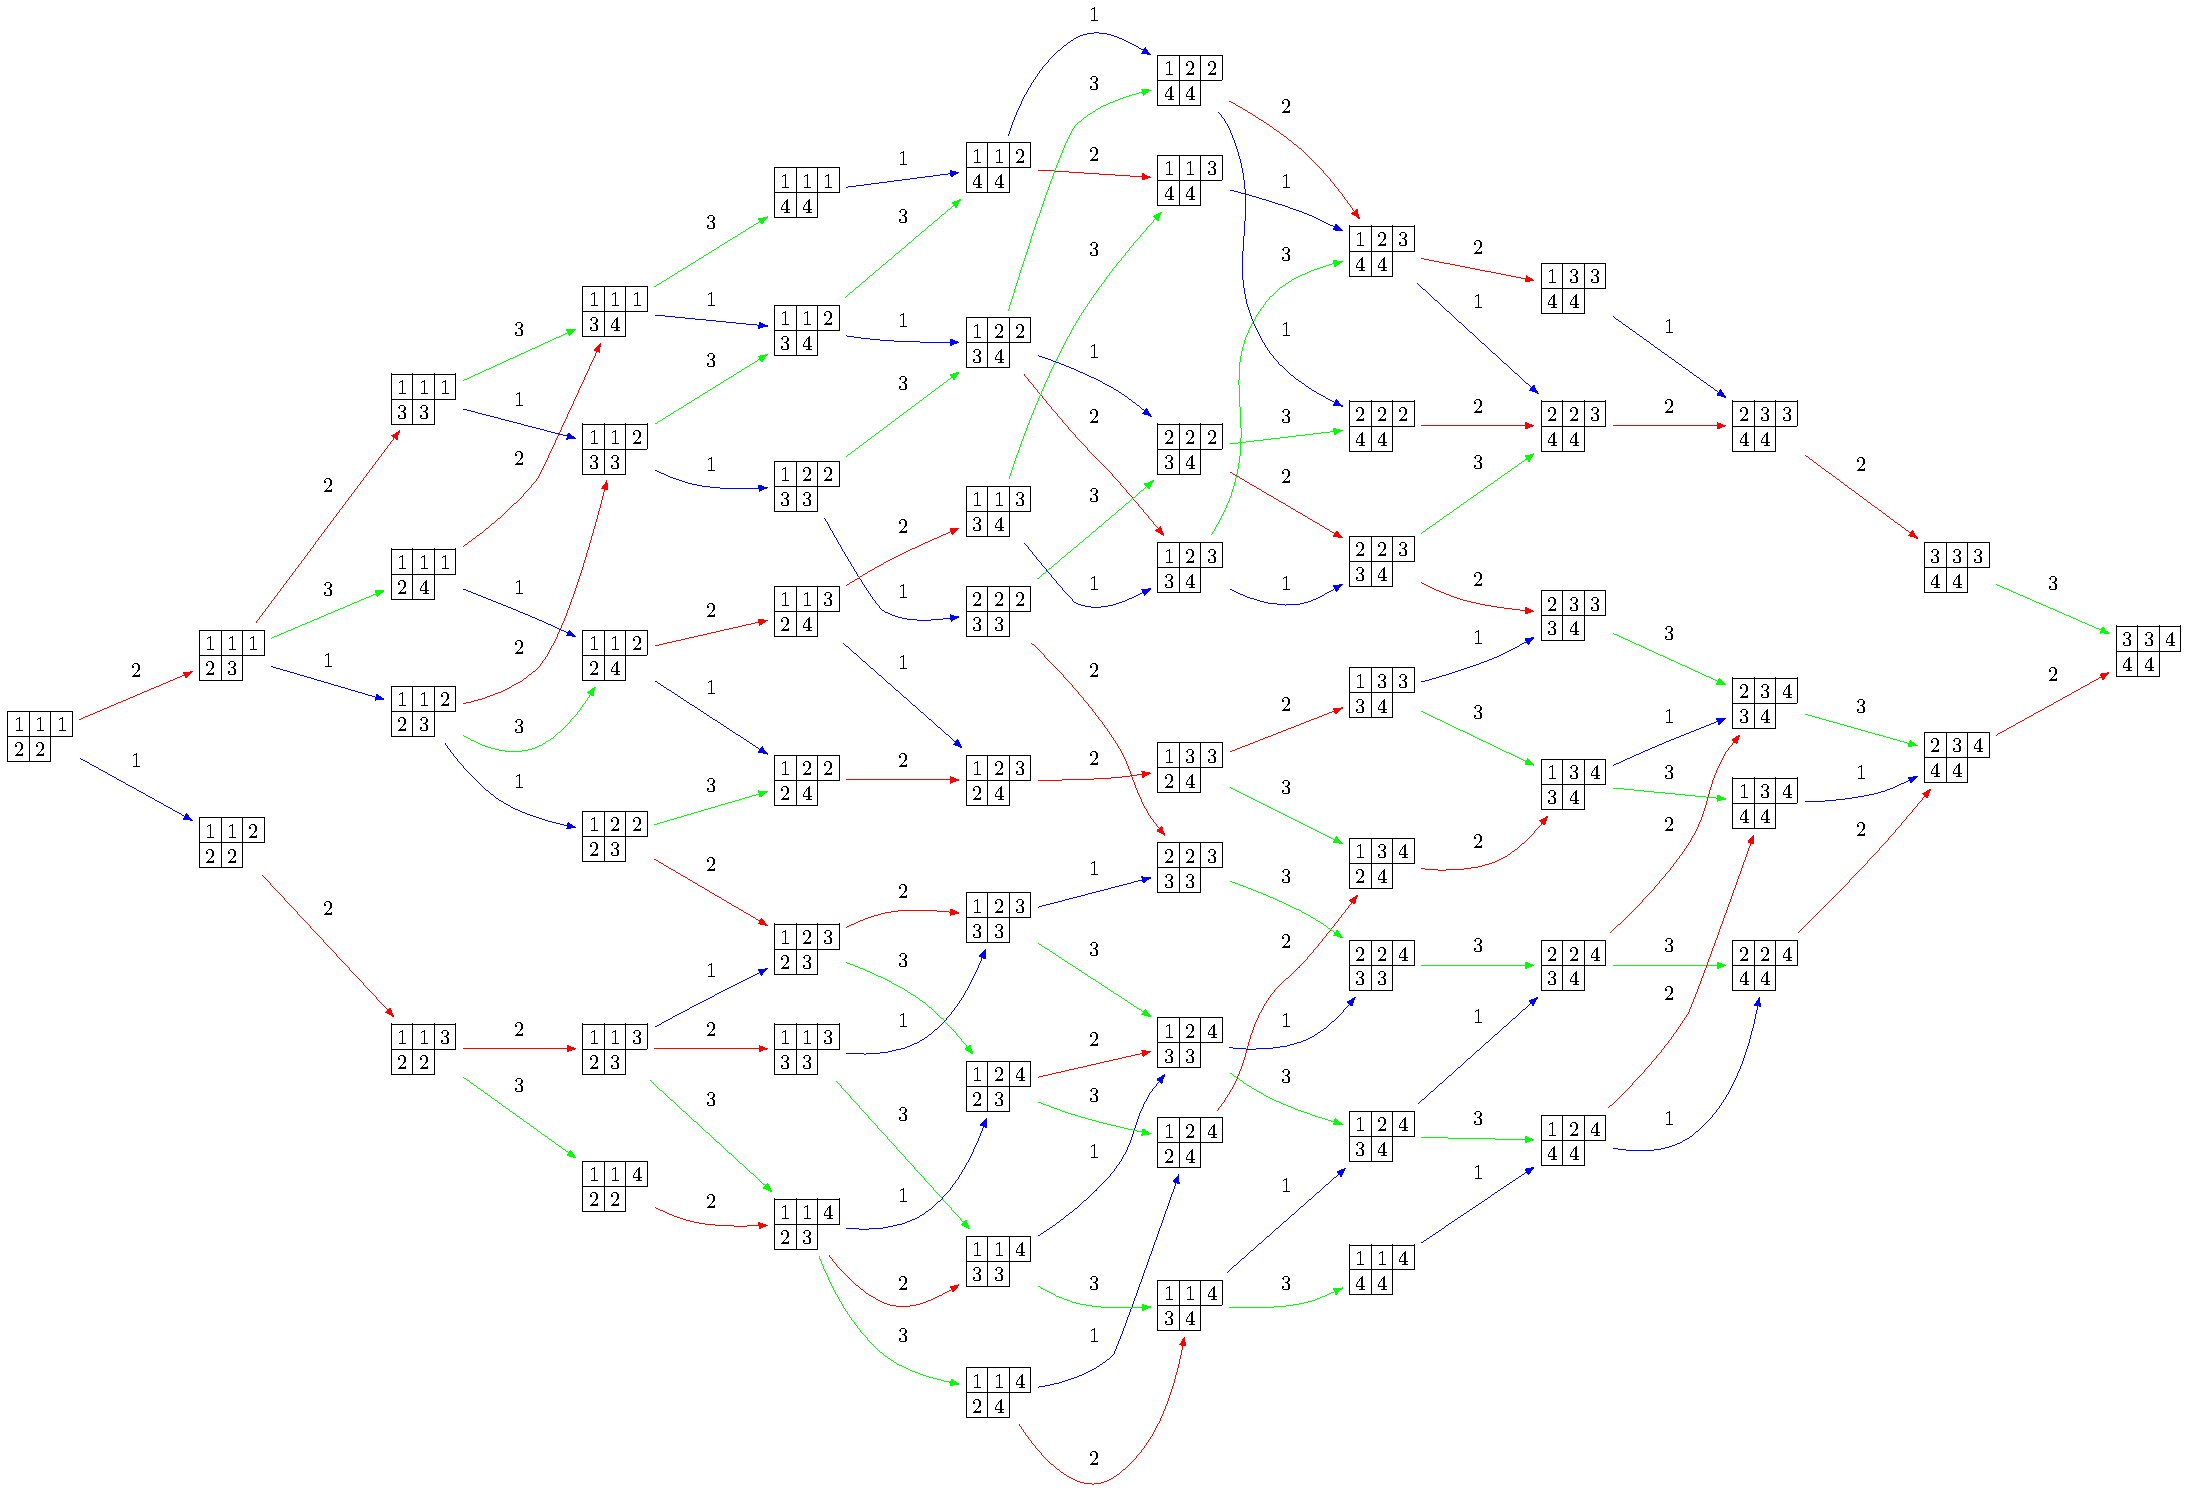
\includegraphics[width=\columnwidth]{Pictures/crystal-A3-32}}
\end{frame}

\begin{frame}{\fr{Objets géométriques}\en{Geometric objects}}
  \centerline{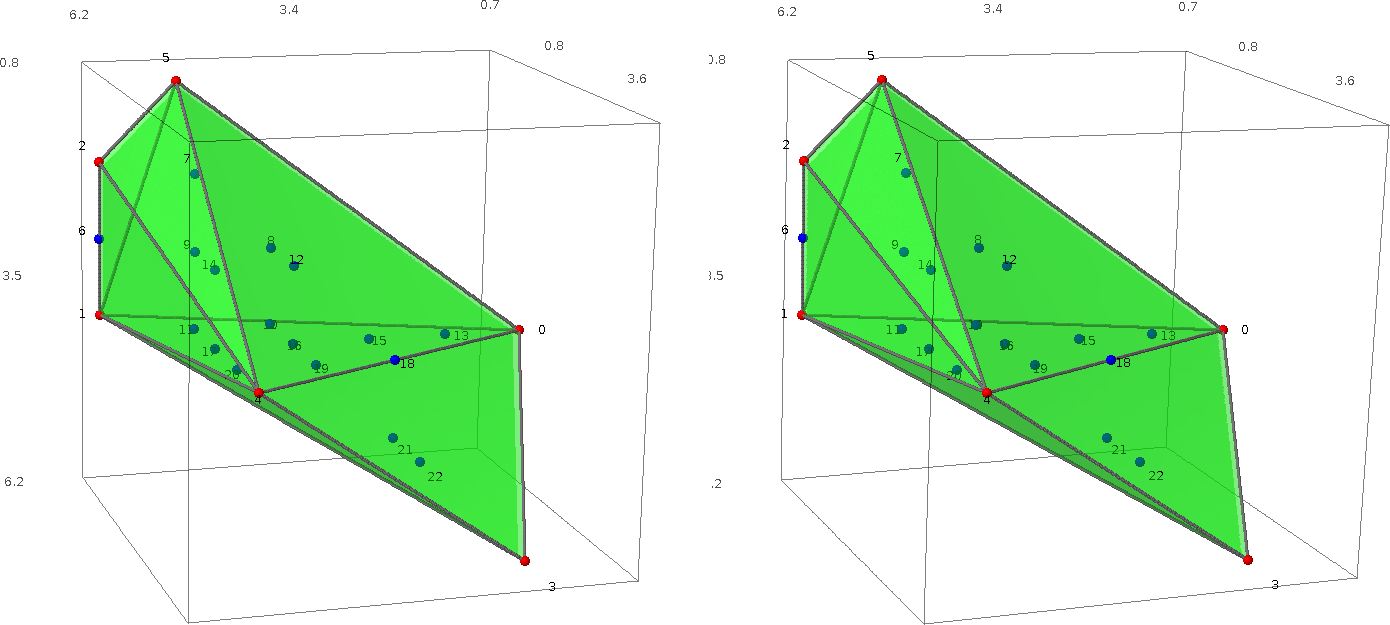
\includegraphics[height=.4\textheight]{Pictures/polytope.png}}

  \centerline{\includegraphics[height=.5\textheight]{G2-alcove-path}\qquad
    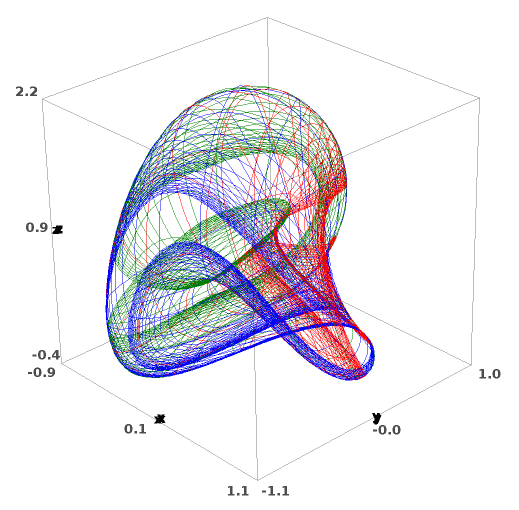
\includegraphics[height=.5\textheight]{manifold.png}}
\end{frame}

\begin{frame}{
    \fr{\Sage: une bibliothèque large\\ d'objets mathématiques et d'algorithmes}
    \en{\Sage: a large library of mathematical objects and algorithms}
  }
  \begin{itemize}
  \item 1.5M
    \fr{lignes de code/doc/tests (Python/Cython)}
    \en{lines of code/doc/tests (Python/Cython)}
    \\
    \fr{+ dépendances}
    \en{+ dependencies}
  \item 1k+ types \fr{d'}\en{of } objets
  \item 2k+ \fr{méthodes and fonctions}\en{methods and functions}
  \item 200 \fr{contributeurs réguliers}\en{regular contributors}
  \end{itemize}
  \pause
  \begin{block}{\fr{Problèmes}\en{Problems}}
    \begin{itemize}
    \item \fr{Comment structurer cette bibliothèque?}
      \en{How to structure this library}
    \item \fr{Comment guider l'utilisateur}
      \en{How to guide the user}
    \item \fr{Comment garantir la cohérence, la robustesse?}
      \en{How to promote consistency and robustness?}
    \item \fr{Comment éviter les duplications?}
      \en{How to reduce duplication?}
    \end{itemize}
  \end{block}
\end{frame}

\begin{frame}{\Sage's large hierarchy of classes}

  \textbf{Model math concepts}: Finite sets, Groups, Fields, Graphs, ...

  By a \textbf{{\only<2>{\color{red} large }\only<3->{\color{red} huge }}hierarchy of abstract classes}:

  \begin{bigcenter}
    \only<1>{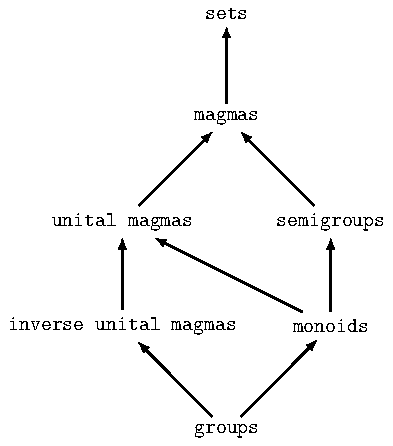
\includegraphics[height=.6\textwidth]{Pictures/Groups-category-graph.pdf}}
    \only<2>{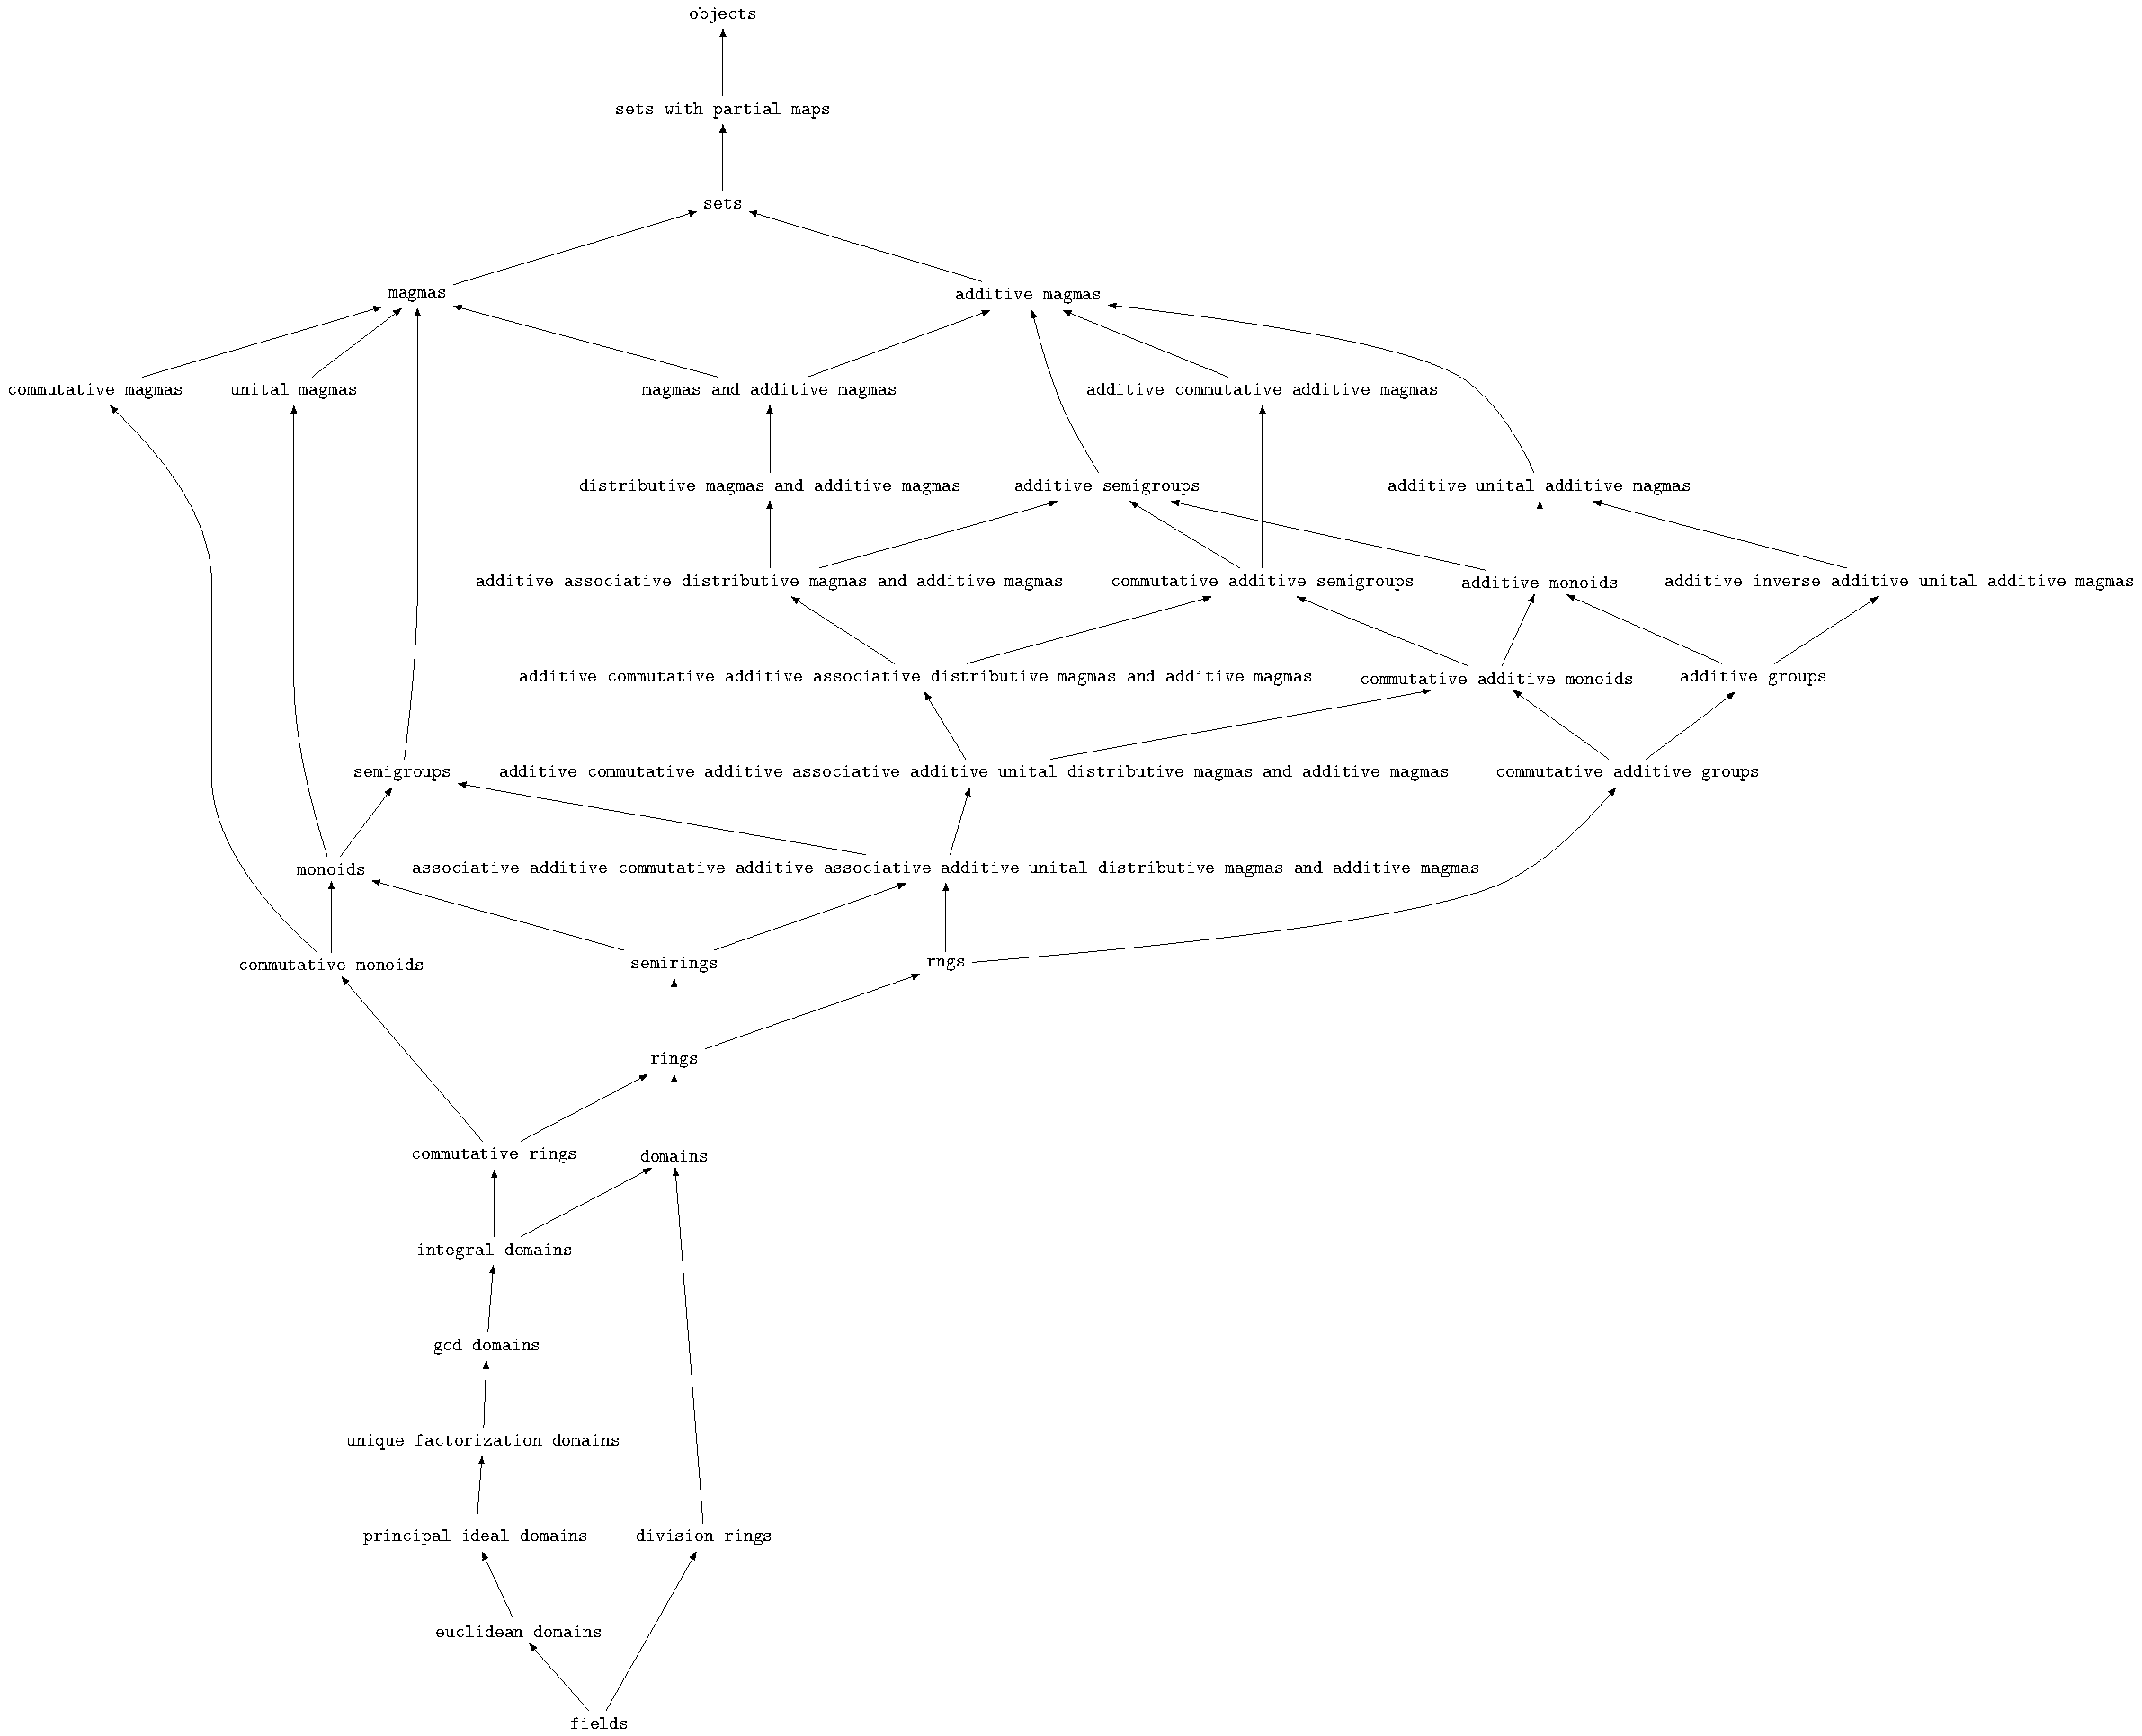
\includegraphics[height=.6\textwidth]{Pictures/Fields-category-graph.pdf}}
    \only<3->{
\includegraphics[width=1.2\textwidth]{Pictures/sage-category-graph.pdf}}
  \end{bigcenter}
  \vfill
  \vfill

  \only<3->{
    \visible<4->{
    Viable because:
    \begin{itemize}
    \item Strong mathematical foundations
    \item Infrastructure: mixins + $\cdots$ + \textbf{C3 under control}!
    \end{itemize}
  }}
\end{frame}

\end{document}

%%% Local Variables: 
%%% mode: latex
%%% TeX-master: t
%%% End: 
